\documentclass{article}
\usepackage[utf8]{inputenc}

\title{CTA200H - Assignment 3}
\author{Louis Branch}

\usepackage{graphicx}
\usepackage{amsmath}
\usepackage{amssymb}
\usepackage{cancel}
\usepackage{mathabx}
\renewcommand{\thesubsection}{\thesection.\alph{subsection}}

\date{May 2022}
\setlength{\parindent}{0em}
\setlength{\parskip}{0.5em}
\renewcommand{\baselinestretch}{1.1}

\begin{document}

\maketitle

\section{Mandelbrot Set}

Display a Mandelbrot set by iterating over: \[f(z) = z^2 + c\]

Where c is a complex value in the form of $c = x + yi$.

The \verb|maldenbrot_set| function accepts two inputs: the number of points between -2 and 2, and the maximum number of iterations to test for the boundary conditions. Higher values for both create a sharper image.

The implementation uses  \verb|numpy.array| for the computation and masking to plot the complex plane with colors based on the number of iterations.

\subsection{Low Resolution}

With 100 points, iterating to a maximum of 20 times we get a low resolution image:

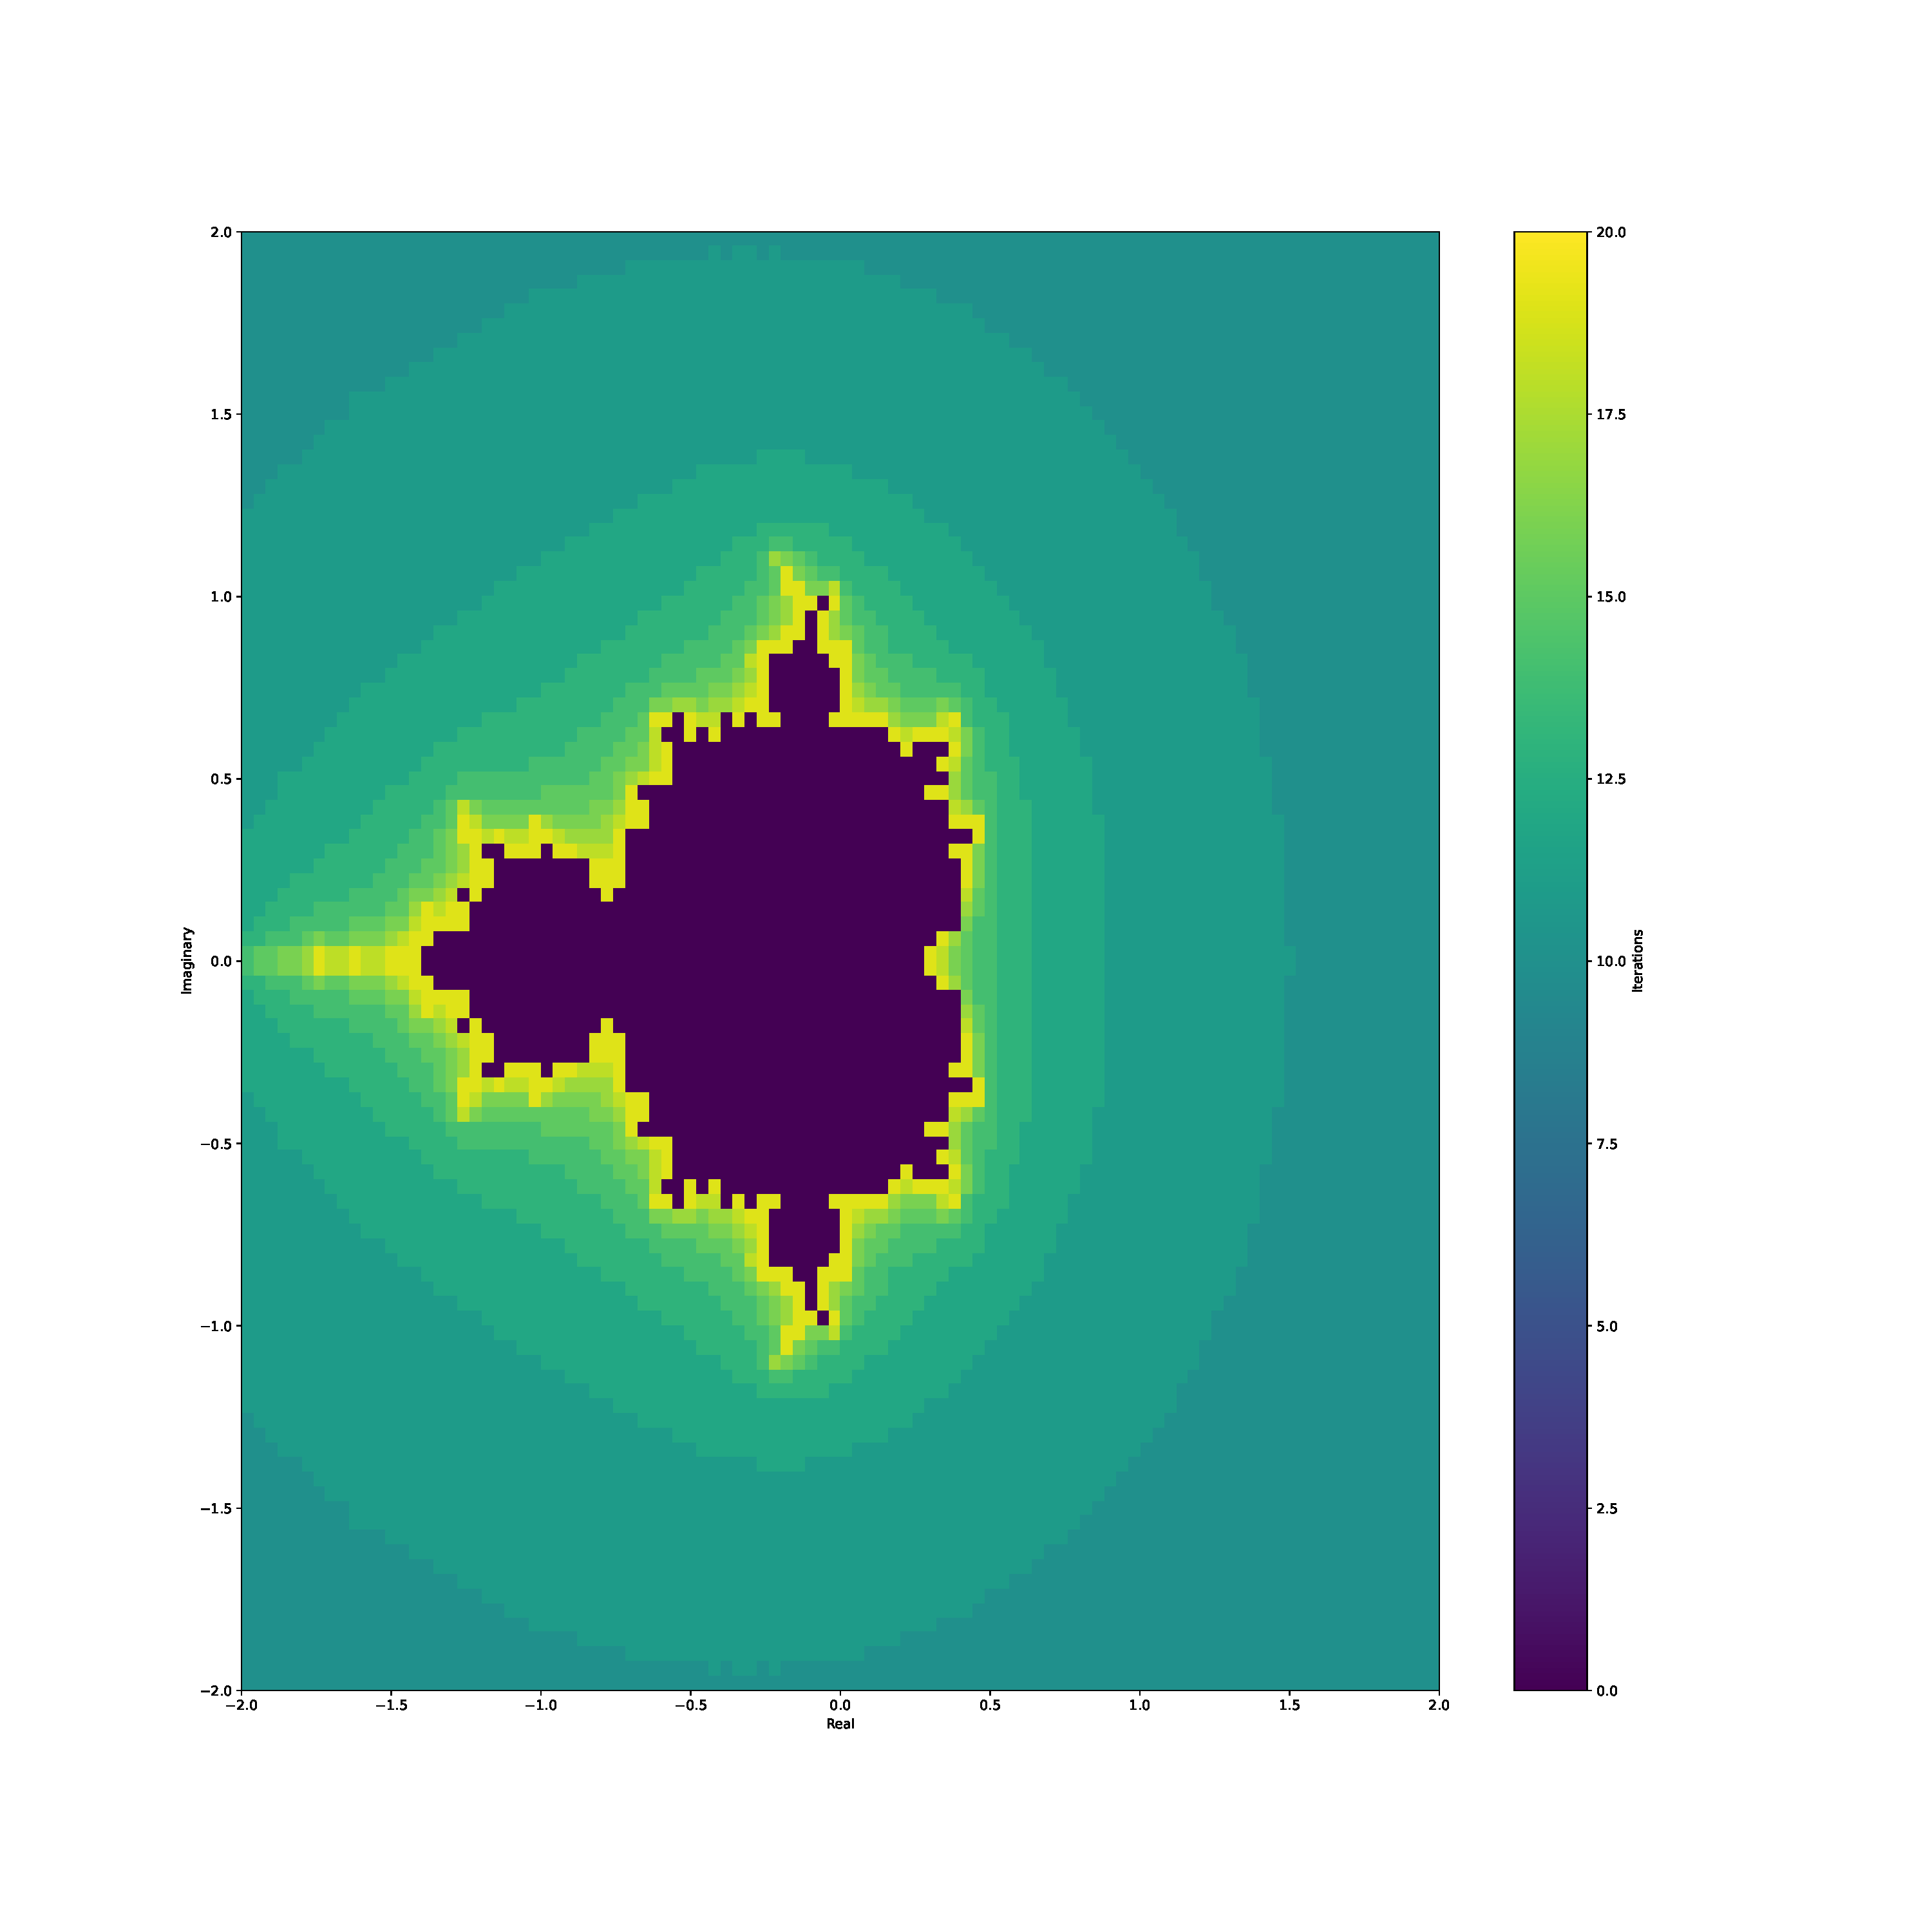
\includegraphics[scale=0.2]{mandelbrot_20.pdf}

\subsection{High Resolution}

With 5000 points, iterating to a maximum of 50 times we get a crispier image:

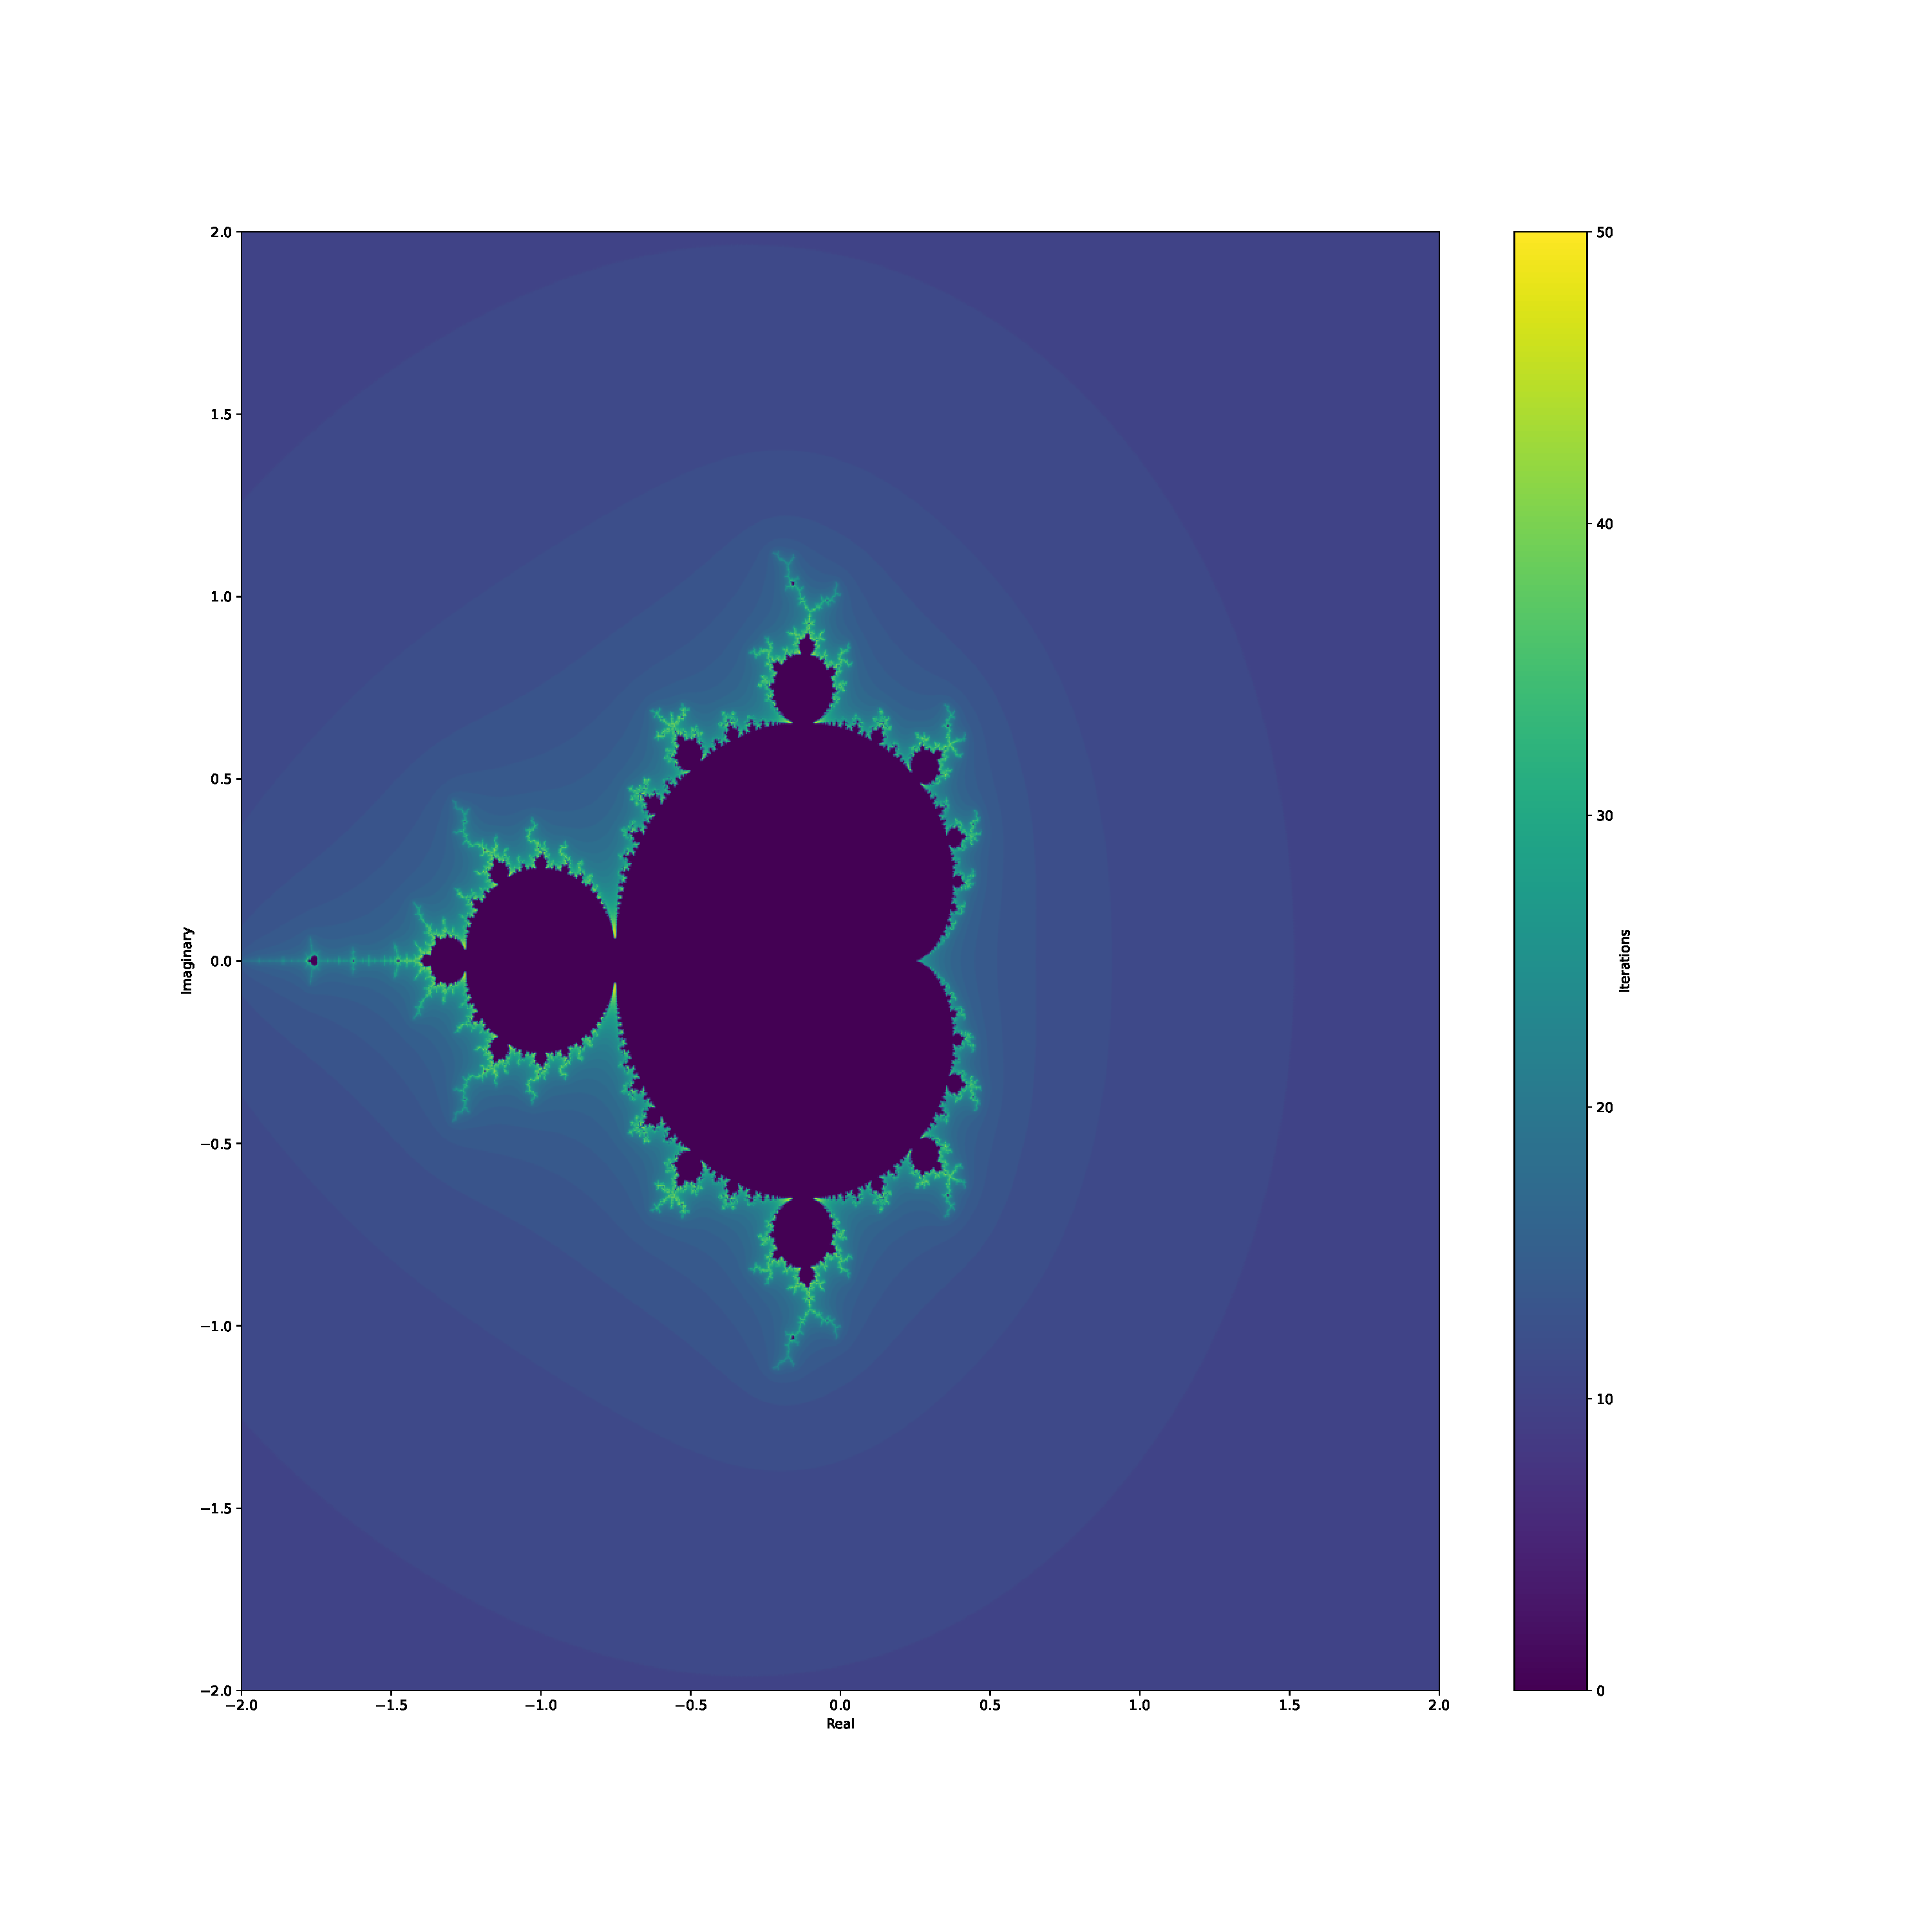
\includegraphics[scale=0.2]{mandelbrot_50.pdf}

\section{Lorenz Equations}

Solve a system of ordinary differential equations simulating chaotic effect
in the atmosphere with initial conditions $W$ in a time frame of 60 seconds.

Lorenz used the following constants:
\begin{align*}
    \sigma &= 10\\
    \beta &= \frac{8}{3}\\
    \rho &= 28
\end{align*}

and initial conditions $W = [0, 1, 0]$.

\subsection{Y(t)}

Display 3 plots as Y as a function of time for half of the period (30 s). Each plot spans 1000 iterations and an iteration is defined as $\frac{time}{\Delta t}$.

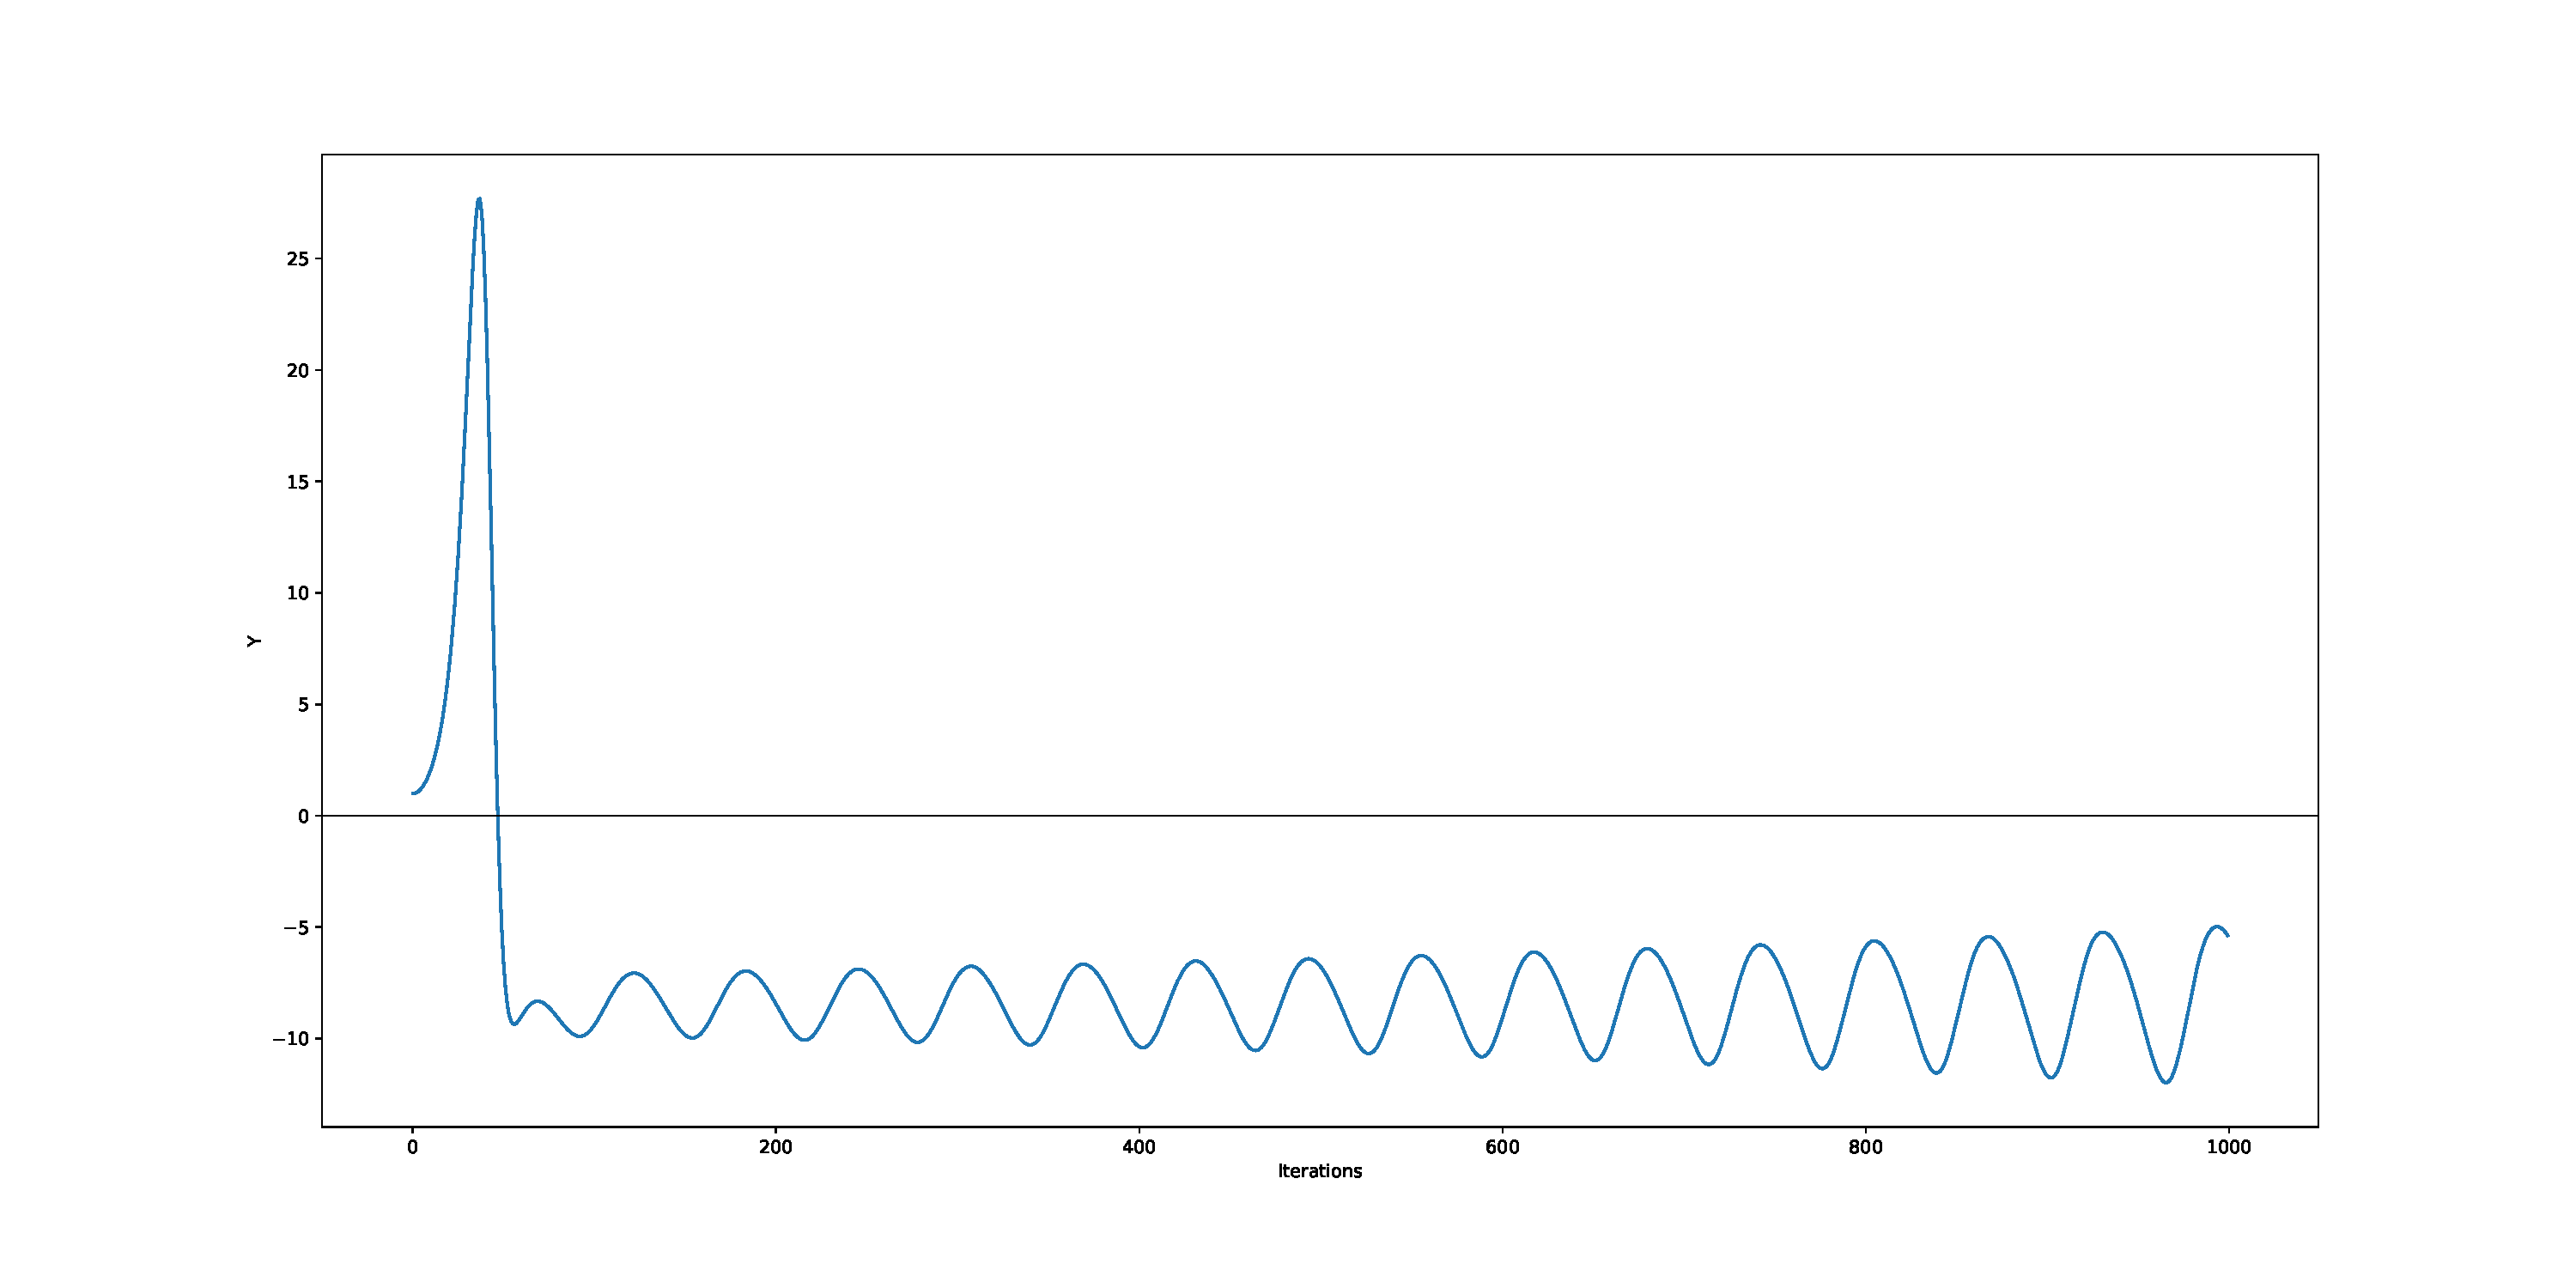
\includegraphics[scale=0.2]{lorenz_1.pdf}

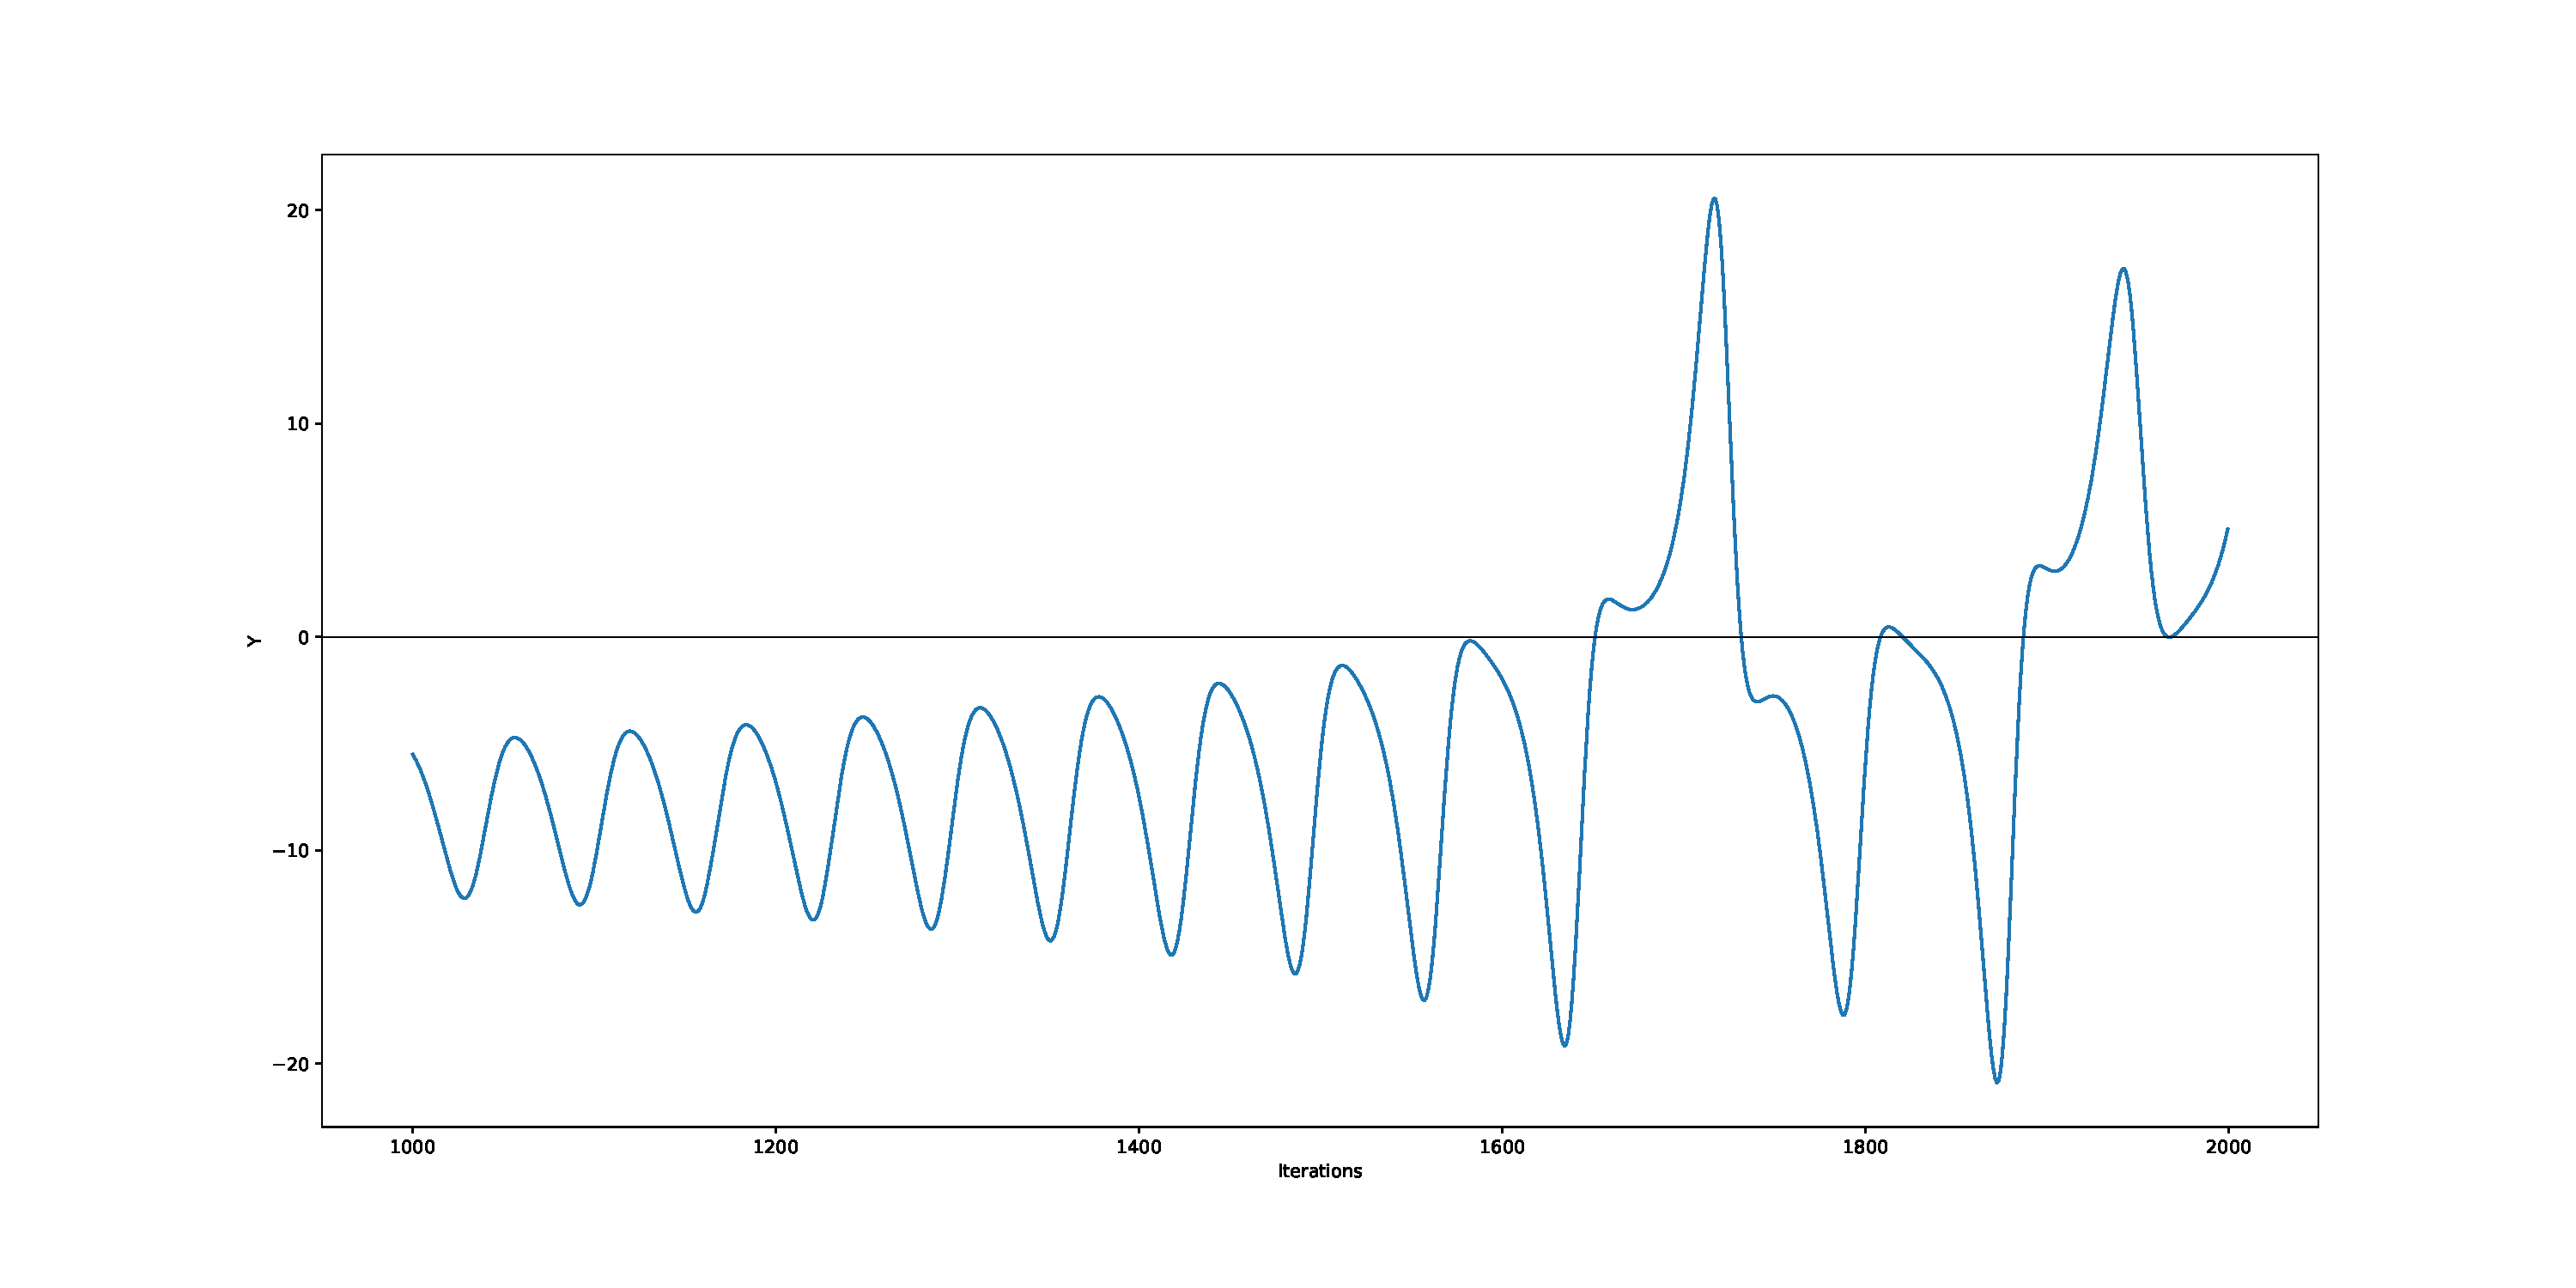
\includegraphics[scale=0.2]{lorenz_2.pdf}

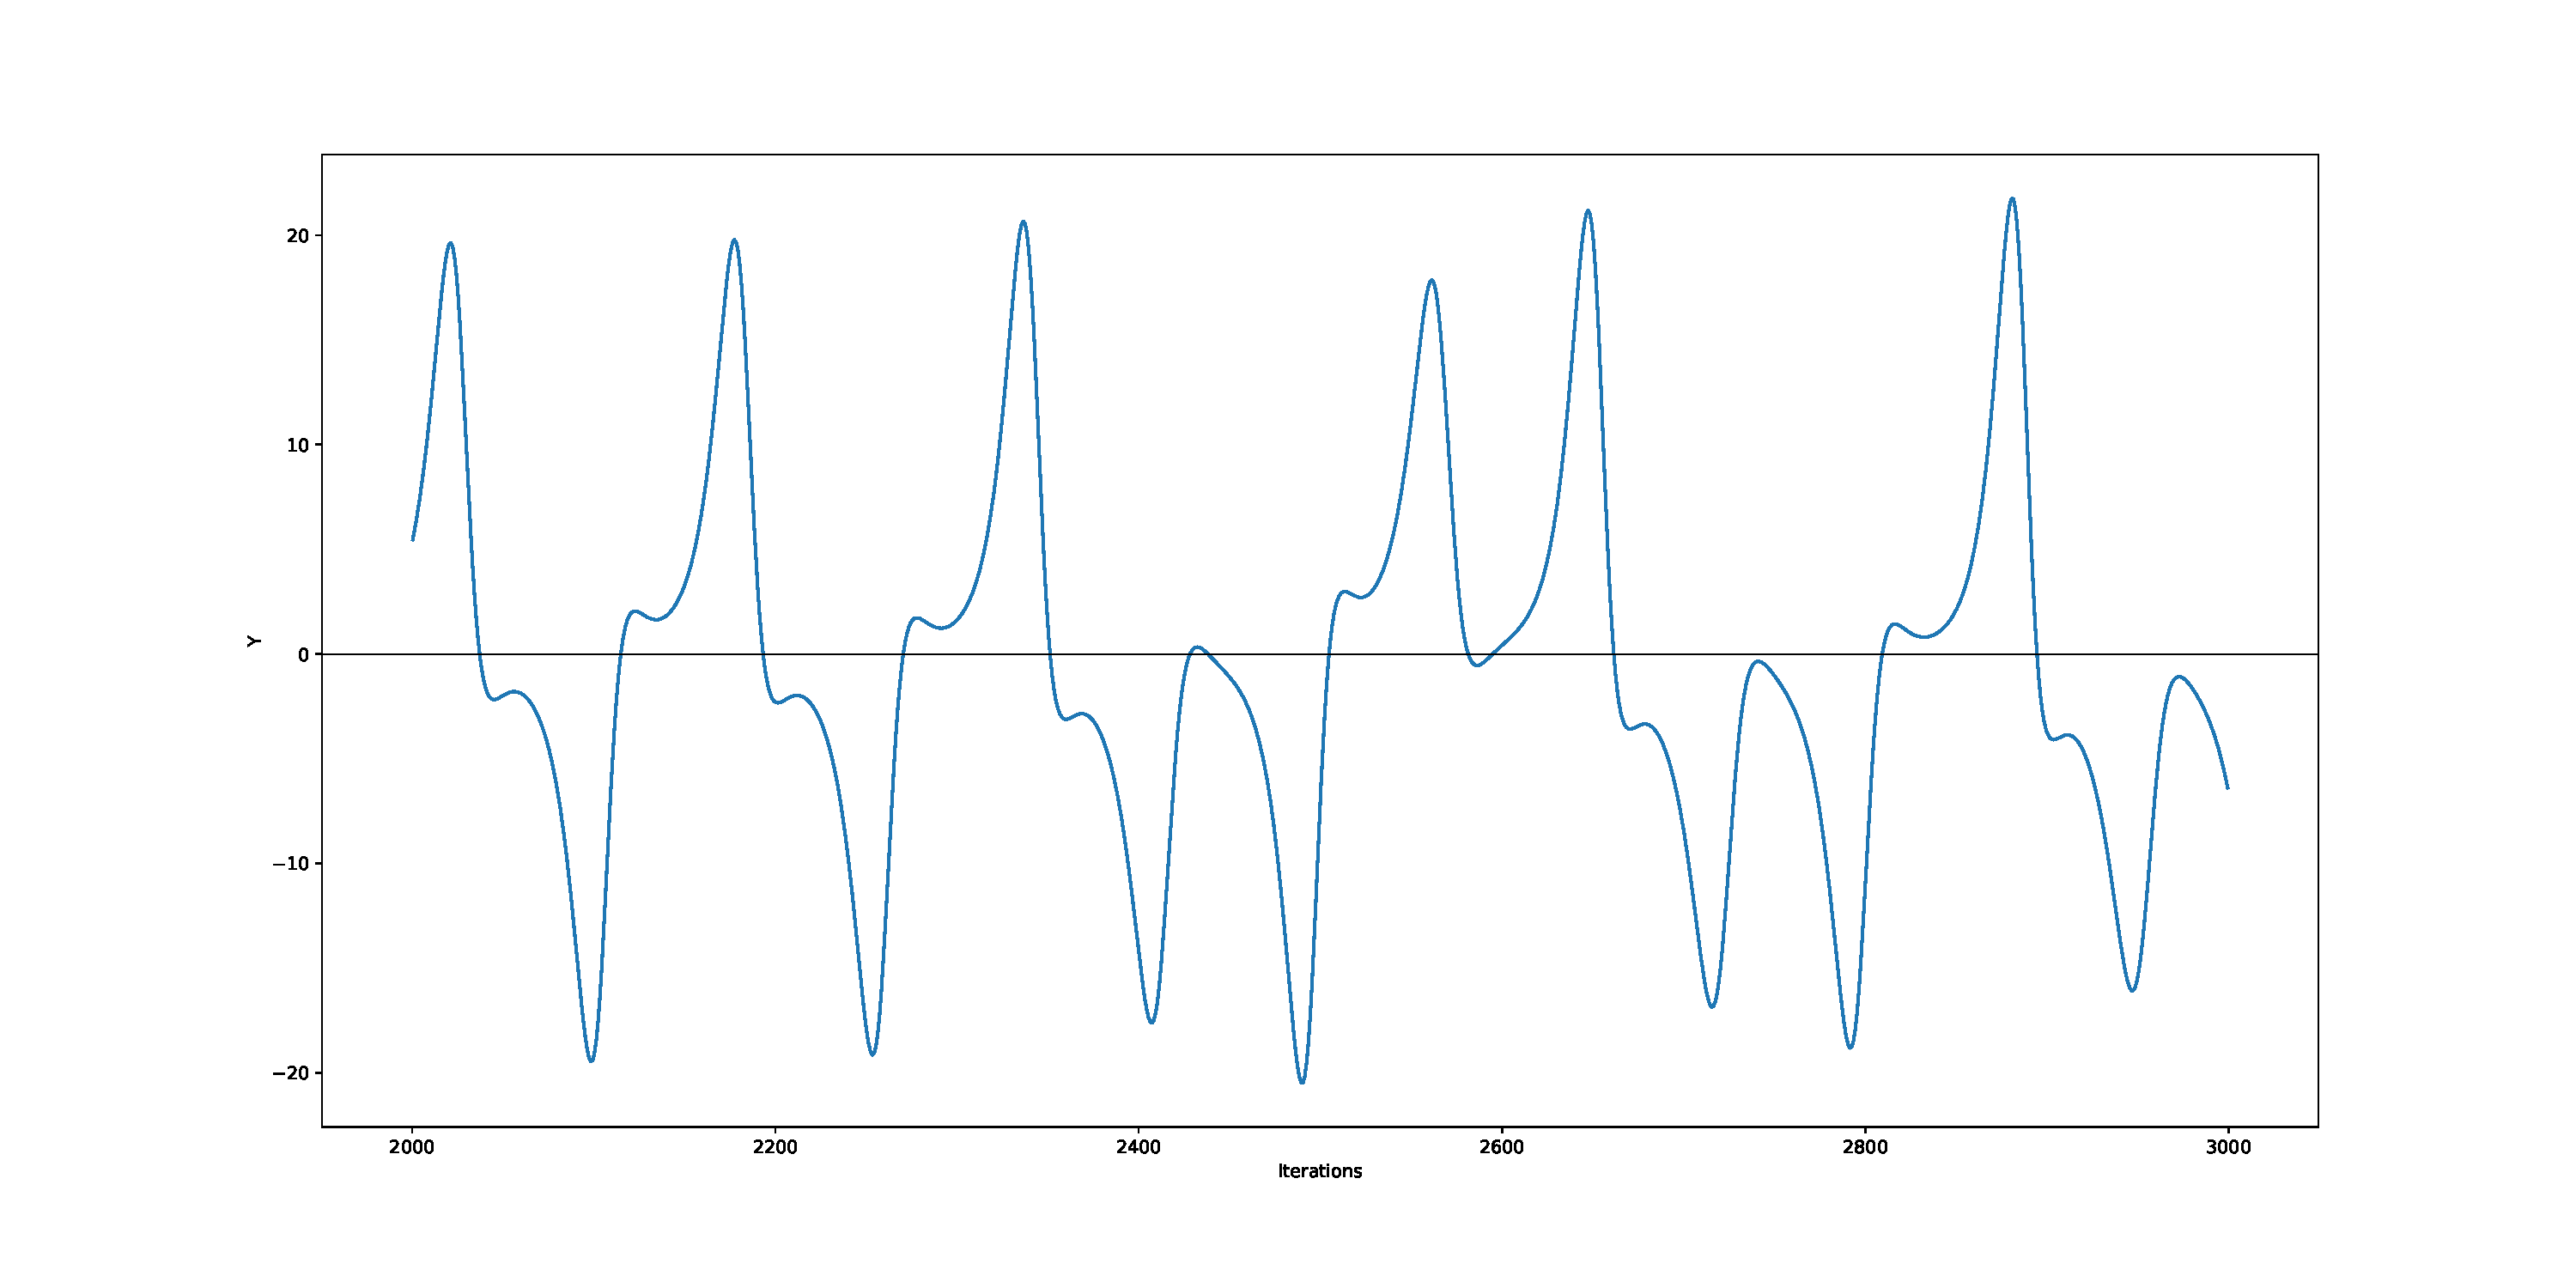
\includegraphics[scale=0.2]{lorenz_3.pdf}

\subsection{Z(Y), X(Y), Z(X)}

Using a subset of the initial space, display Z as a function of Y:

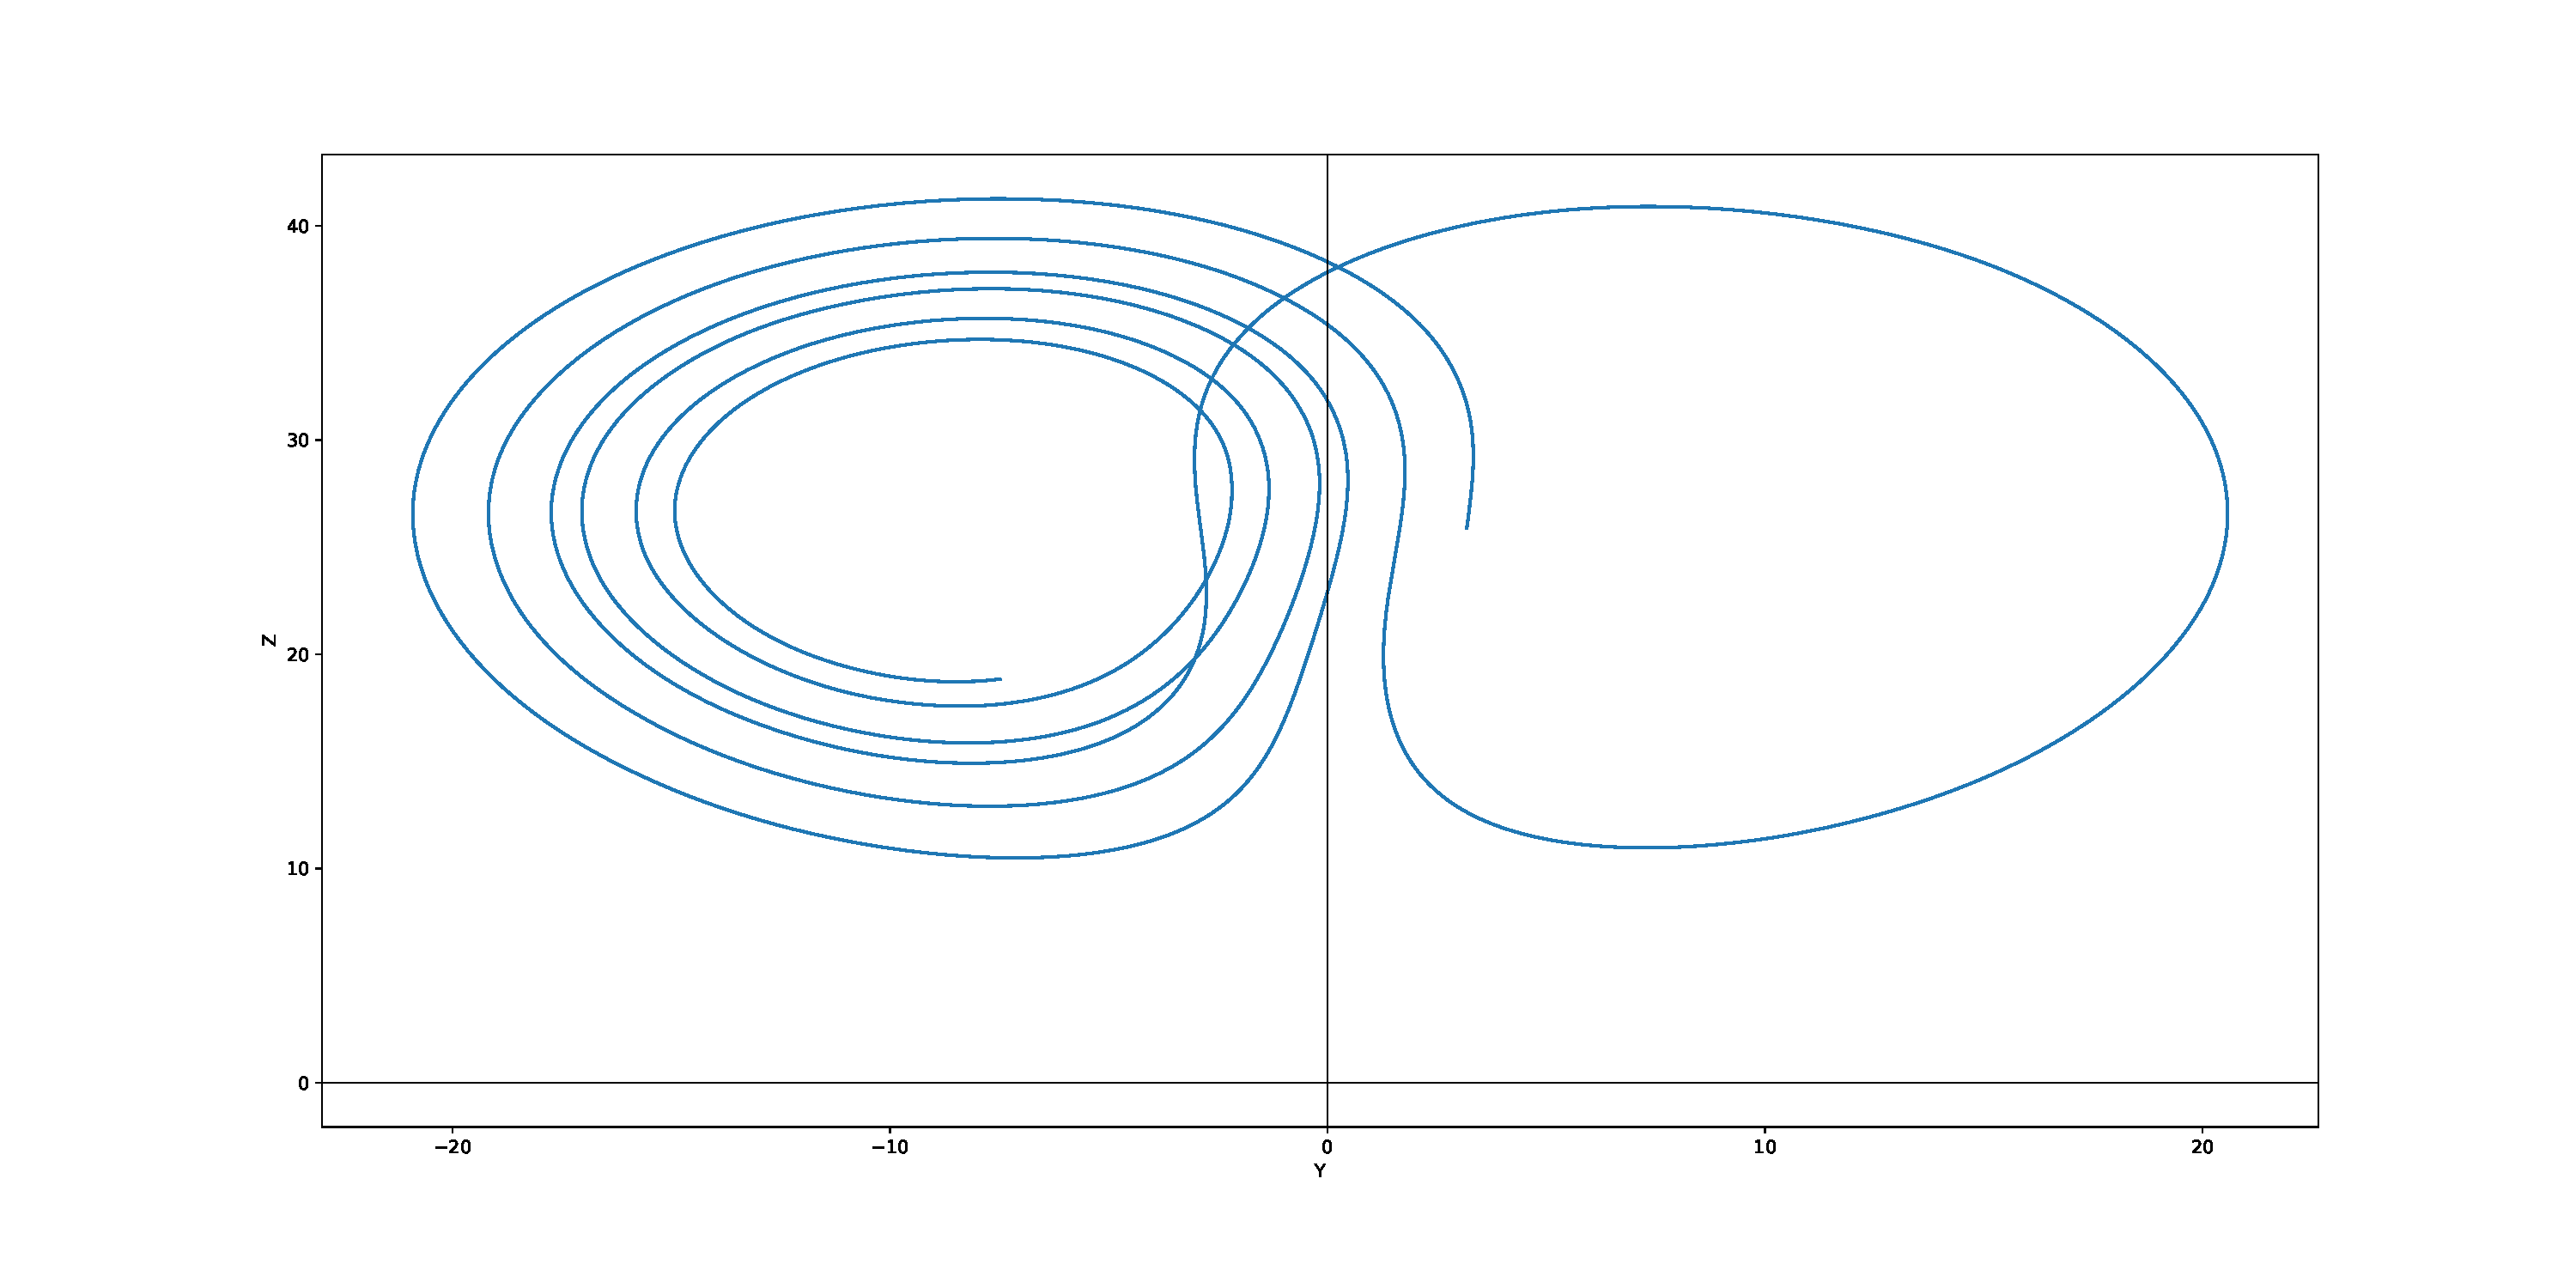
\includegraphics[scale=0.2]{lorenz_4.pdf}

X as a function of Y, the X-axis is inverted to match the graph on the original paper:

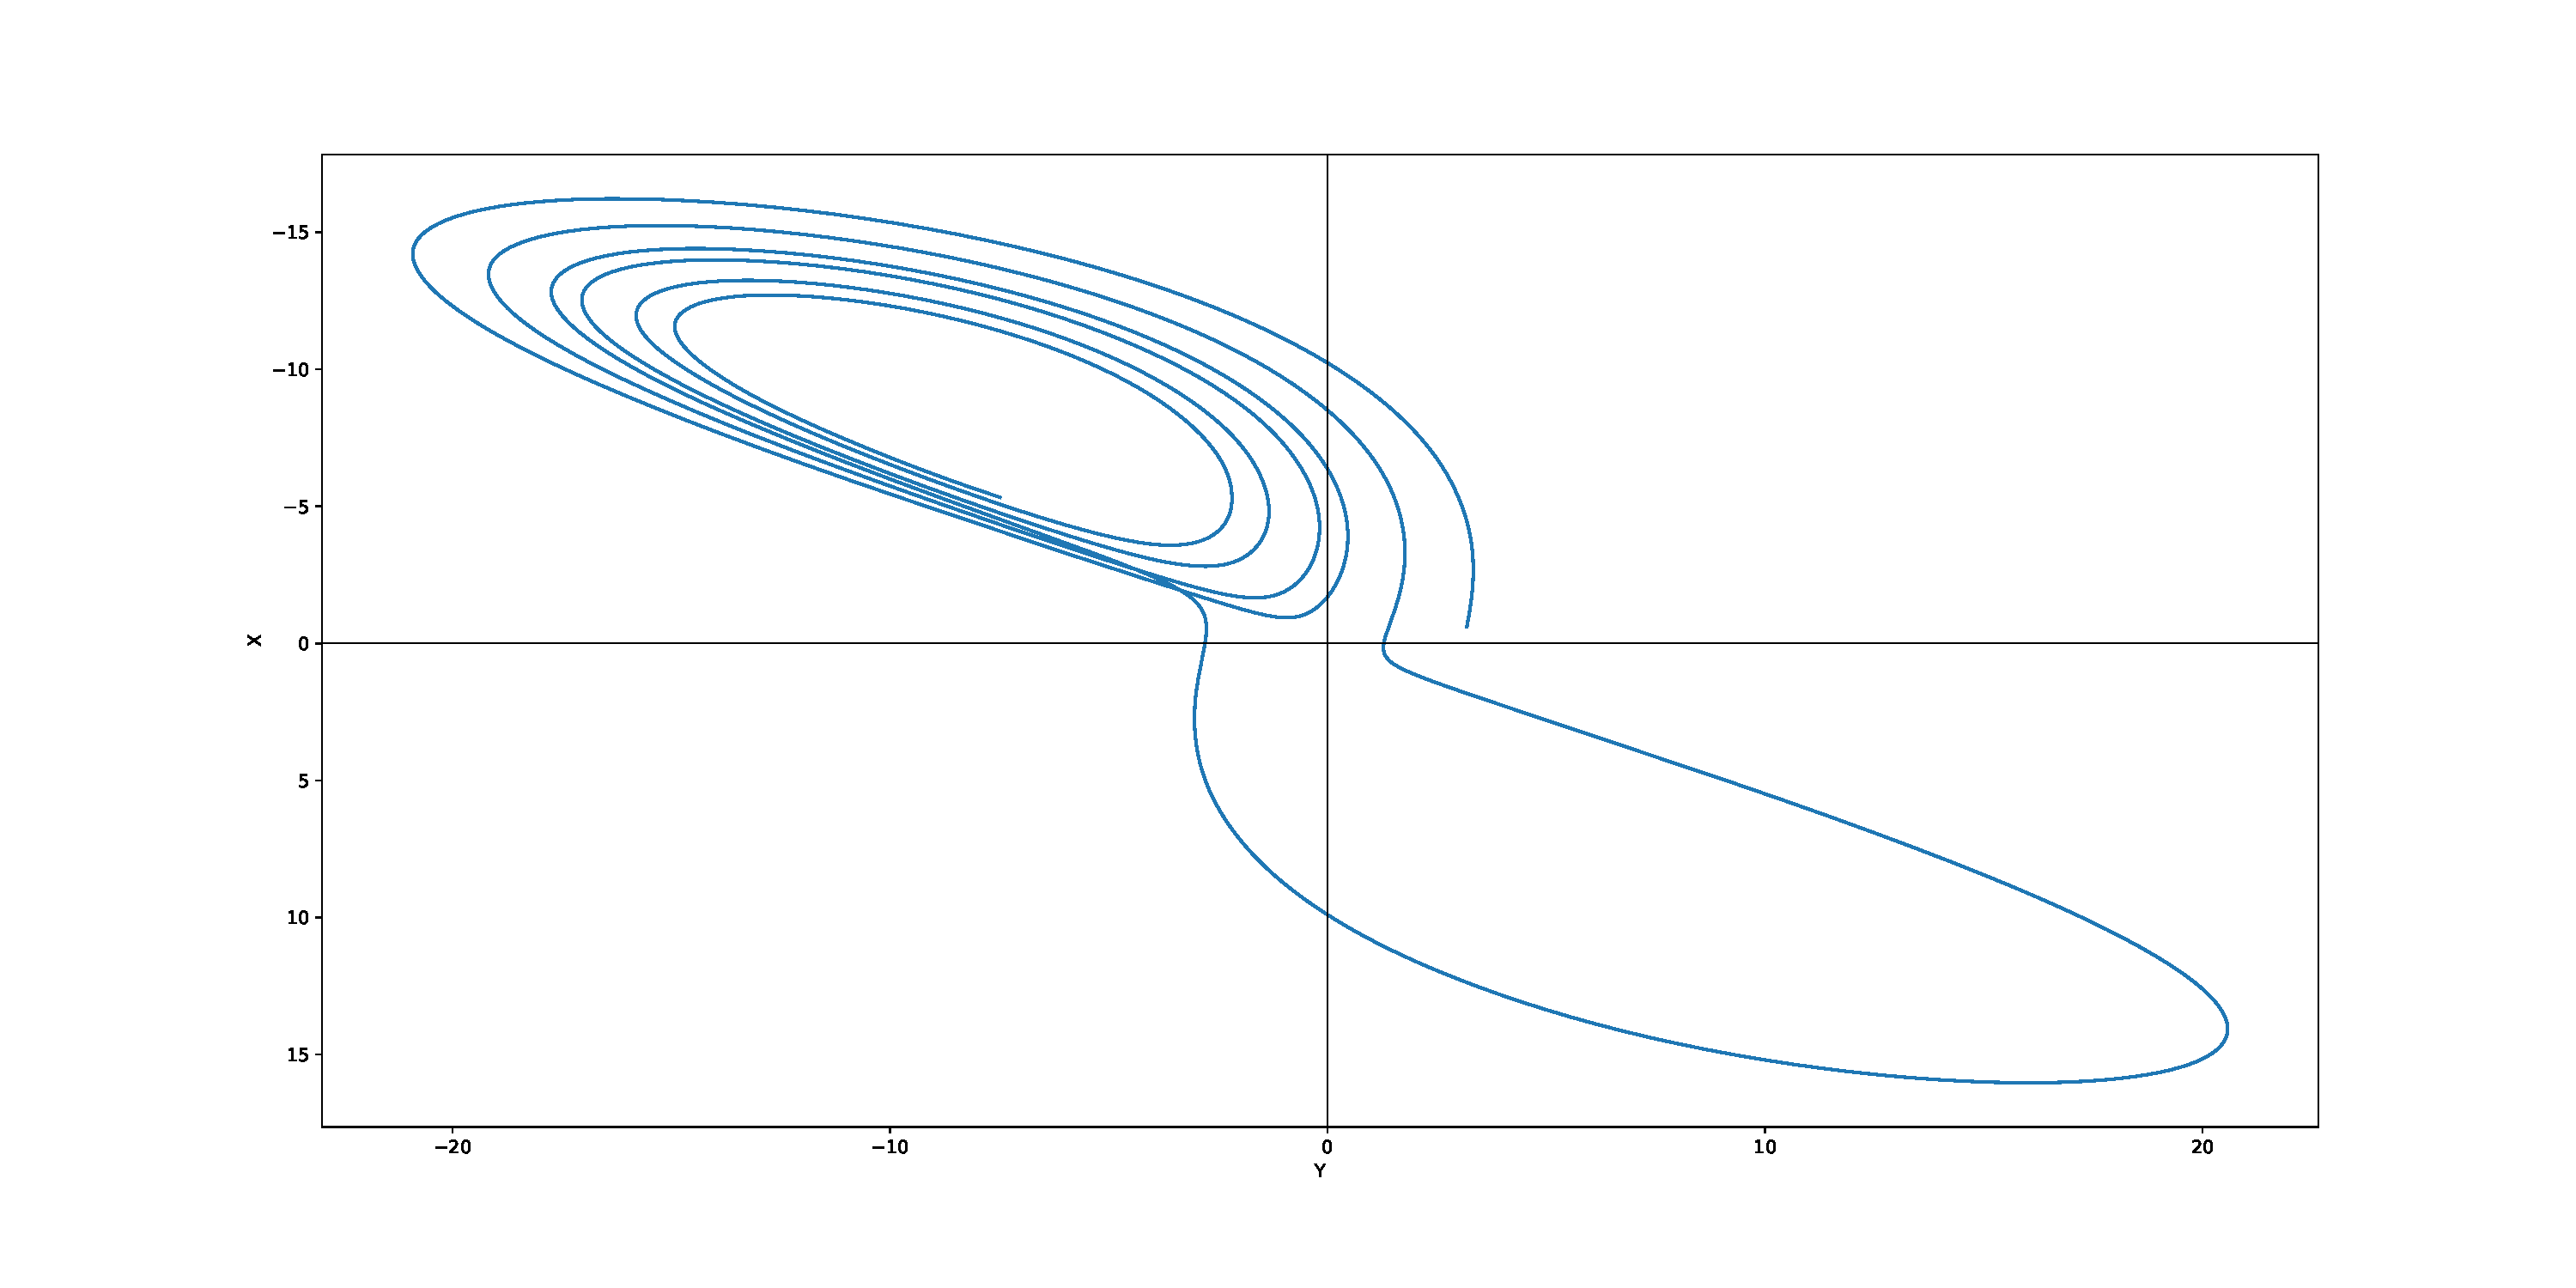
\includegraphics[scale=0.2]{lorenz_5.pdf}

And for the famous "Butterfly Effect", Z as a function of X:

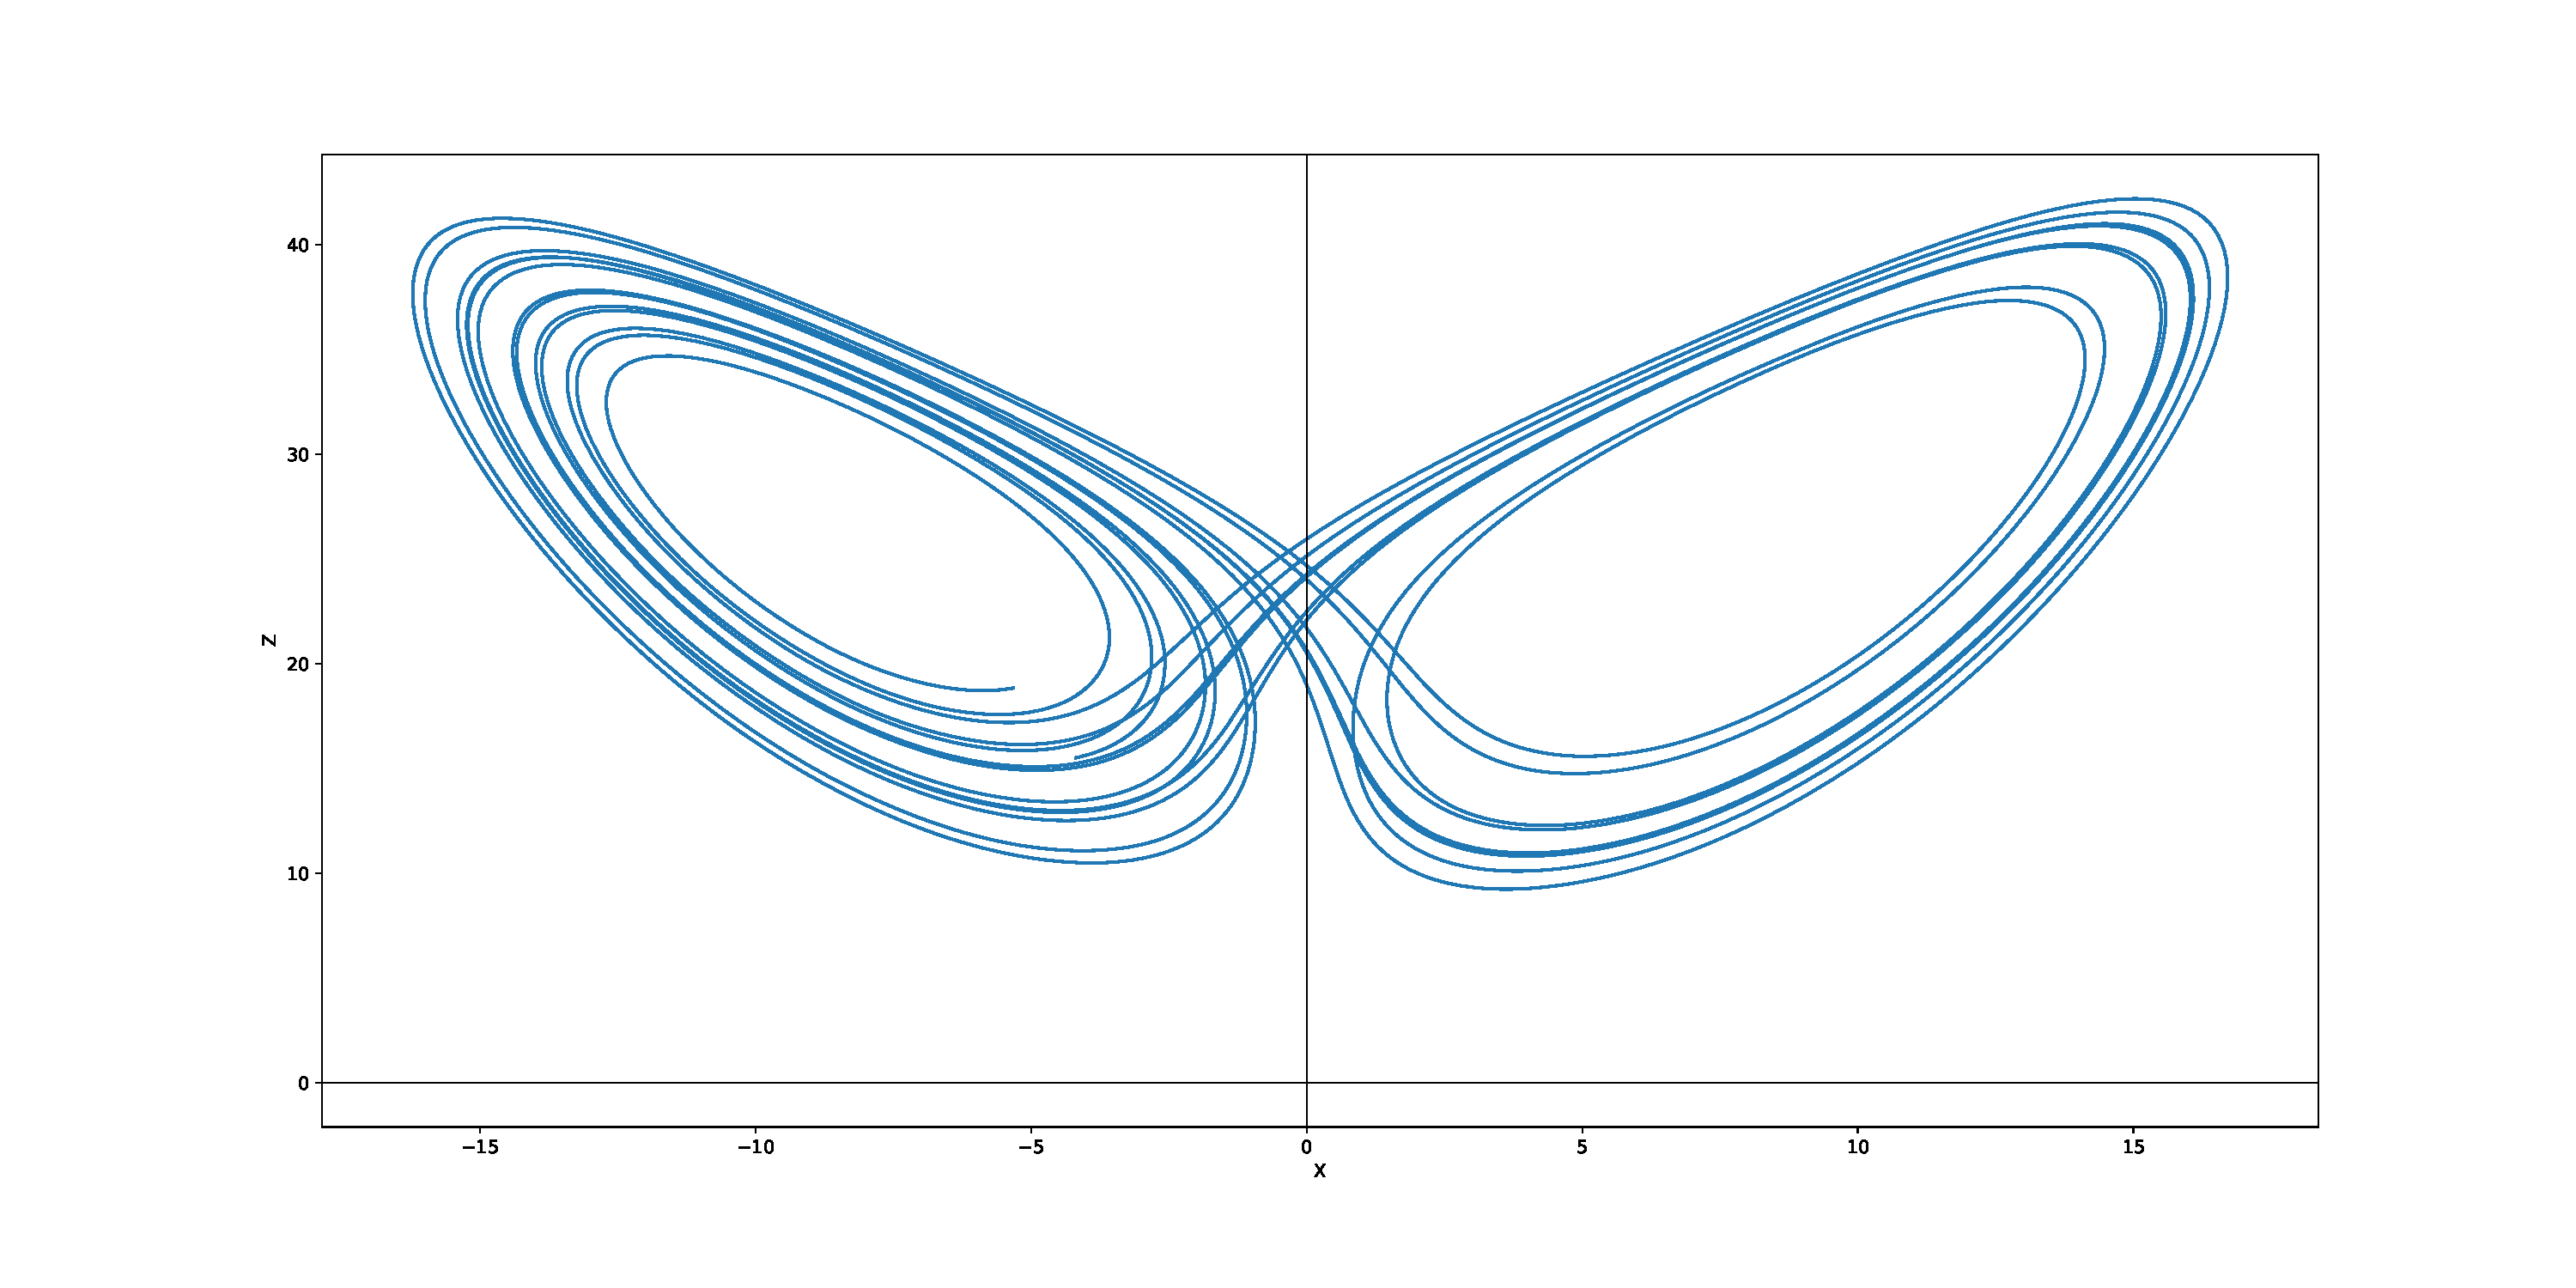
\includegraphics[scale=0.2]{lorenz_6.pdf}

\subsection{Different initial conditions}

Using different initial conditions $W' = [0, 1.00000001, 0]$, display a semi-log plot with the absolute distance between $W$ and $W'$ over time.

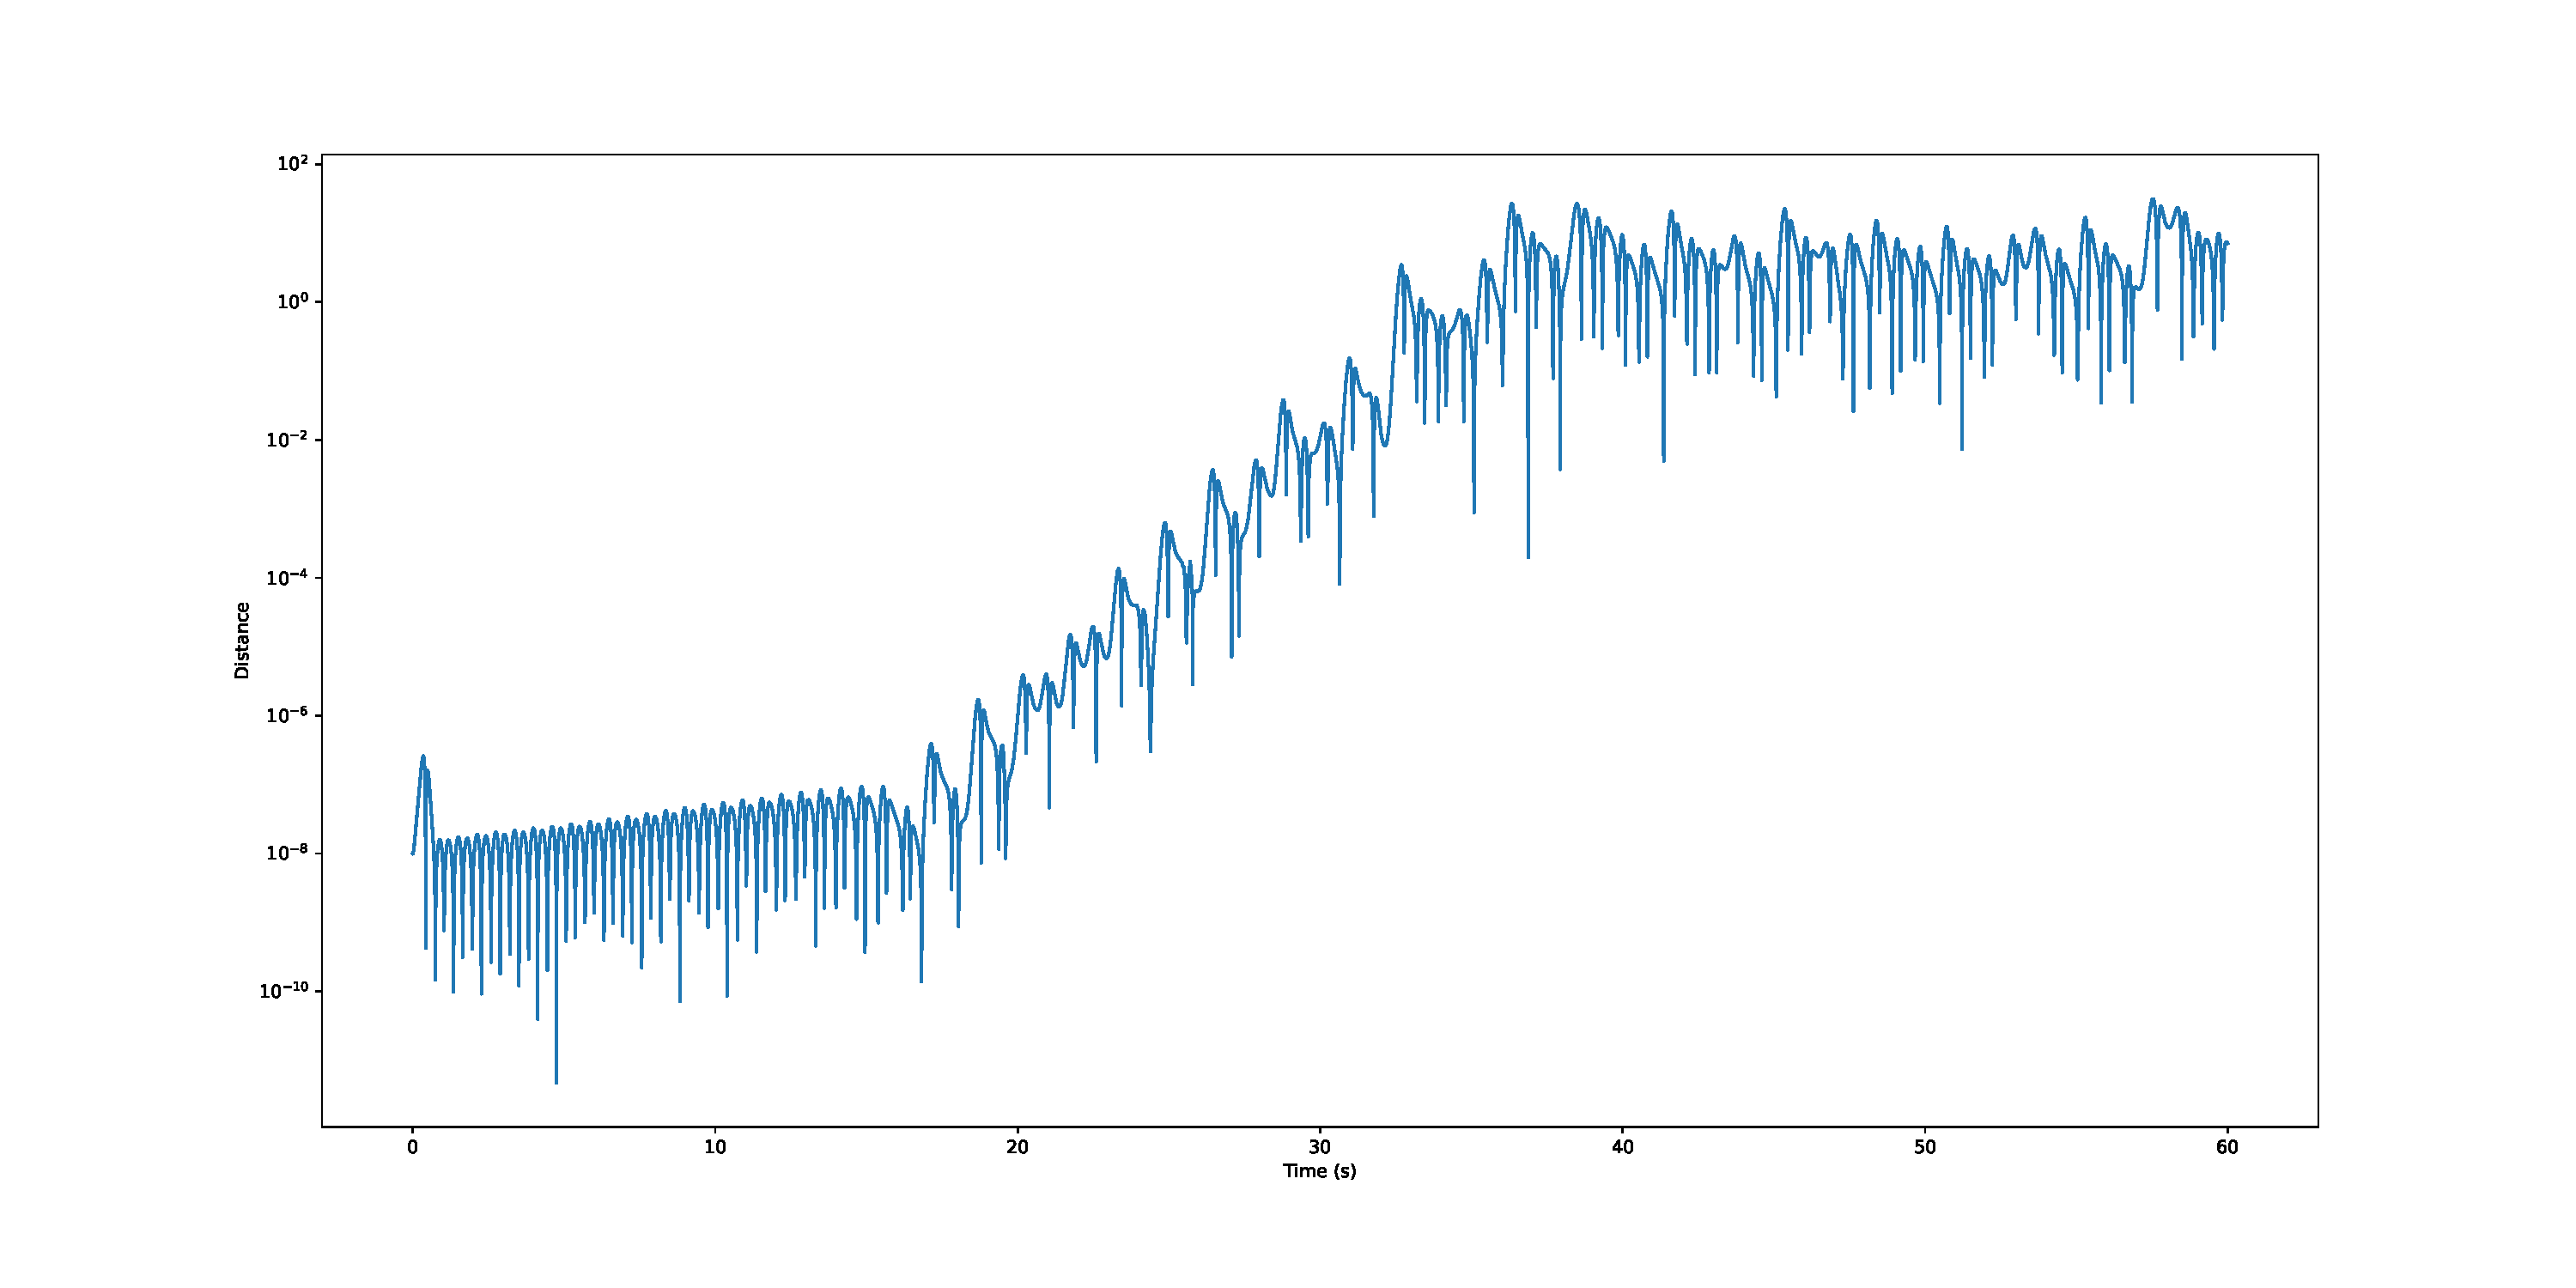
\includegraphics[scale=0.2]{lorenz_7.pdf}


\end{document}
